\chapter{Resultados}
\label{chap:result}

As funcionalidades do sistema de percepção foram validades a partir de duas etapas de teste. Os testes unitários buscam a validação do funcionamento de cada sensor individualmente enquanto os testes integrados validam o funcionamento dos sistemas e funcionalidades. A descição dos testes realizados e dos resultados obtidos por eles está descrita abaixo.

%--------- NEW SECTION ----------------------
\section{Testes unitários}
\label{sec:testu}

    \subsection{Câmera Térmica}
    
    A câmera térmica se comunica por VOSPI. Logo, foi necessário utilzar um driver para converter os dados da câmera e disponibilizá-los para USB. Foi utilizada a placa de interface Nucleo STM32F401RE com o driver disponibilizado por \citeonline{groupgets}. 
    
    O driver apenas coleta os frames e envia para a USB seguindo o seguinte padrão de mensagem:
    
    \begin{figure}[!ht]
    	\centering
    	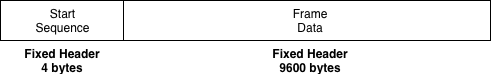
\includegraphics[width=14cm]{Figures/frame_msg.png}
    	\caption{Mensagem do frame da câmera} \label{framemsg}
	\end{figure}
    
    Na qual cada \textit{pixel}, dois \textit{bytes}, foi convertido para uma escala de cinza de 8-bit através de um algoritmo em python no computador, necessária para trabalhar com a biblioteca de processamento de imagens OpenCV.
    
    Após isso a imagem era reconstruida para verificar o funcionamento da câmera.
    
    \subsection{Sonar EZ-1}
    O sonar EZ-1 da MaxBotix possui saída analógica, desta forma para cada distância medida existe um valor de tensão associado no pino AN do sonar. Para testar o sensor de proximidade foi utilizada uma das portas analógicas da Phidgets que possui um pino de VCC, um de GND e um pino Analógico. Com o driver da phidgets instalado no computador e funcionando foi necessário apenas conectar os pinos de VCC, GND E AN do sensor nos pinos correspondentes da Phidgets e compilar um código para leitura de tensão - disponibilizado no próprio site da Phidgets - no terminal do computador. 
    
    Ao compilar o código você recebe no intervalo de 10s todas as leituras de tensão efetuadas no sensor. Notamos que ao afastar o obstáculo do sonar o valor de tensão aumentava e quando aproximavamos o obstáculo o valor de tensão diminuia, indicando a linearidade do sensor e validando o seu funcionamento.
    
    \subsection{Sensor de Proximidade}
    O sensor de proximidade possui um LED vermelho em sua estrutura, toda vez que o sensor identifica a presença de algum objetivo o LED ascende. Por isso, o sensor foi alimentado através de uma fonte de tensão ajustada para 5V e o LED foi observado. Ao colocar um objeto na frente do sensor a luz ascendia e ao retirar o objeto a luz apagava, indicando o pleno funcionamento do sensor.
    
    \subsection{Sensor de corrente}
    
    O sensor de corrente da Phidgets consegue ler valores entre -30 a +30 com resolução de 75mA. Por isso para testar do sensor era necessário uma fonte de corrente com valor maior que 75mA. O circuito utilizado para fornecer essa corrente foi um LED de alto brilho com um resistor de potência em série. A corrente estimada foi de 100mA. Para testar o funcionamento do sensor este precisava ter seus dois canais de entrada conectados em série no circuito e a saída do mesmo foi conectado na porta analógica da Phidgets. A partir do script VoltageInput anteriormente mencionado, foi possível obter os dados de corrente da leitura do sensor. Os dados obtidos foram compatíveis com os valores de corrente real confirmando o funcionamento do sensor. 
    

    \subsection{Smart Charger}
    
    A placa de gerenciamento e carregamento das baterias funciona a partir do protocolo de comunicação SMBus, este protocolo é baseado no protocolo i2c. As informações de tempertatura, tensão, carga entre outras possuem uma codificação. Por isso para comunicar com a placa você precisa escrever uma mensagem para ela contendo o endereço da bateria que você quer ler a informação, o código da informação que você quer ler e entrar com o endereço de memória no qual a informação será escrita.
    
    Foi implementado um código na placa de interface Nucleo STM32L432 para receber as informações provenientes da Smart Charger e disponibiliza-la na USB da placa. Foram lidos os dados de temperatura, carga e tensão. Os dados obtidos foram convertidos para valores em grau celsius, KWh e Volts respectivamente e assim puderam ser validados. 

    \subsection{Sensor de Temperatura }
    
    O sensor de temperatura LM35 é um sensor com saída analógica e com comportamento linear entre a tensão de saída e a temperatura medida. O sensor foi testado em uma das portas analógicas da Phidgets, conectando os pinos de VCC,GND E AN do sensor nos pinos correspondentes na Phidgets e o algoritmo de leitura de tensão foi utilizado para realizar a obtenção de dados. Para simular ambientes quentes e frios, foi medido o valor de tensão de saída para uma sala com ar-condicionado e após isto foi medido a temperatura assoprando o sensor. O valor da tensão de saída aumentou, como o sensor é linear e o valor de temperatura é o valor da tensao de saída multiplixado por 10, foi possível confirmar a coerência dos valores encontrados validando o funcionamento do sensor.
    \subsection{GPS}
    
    O GPS foi testado a partir de um console disponibilizado no próprio site do fabricante. Foi necessário instalar esse console e conectar o GPS na USB do computador. A sua antena também foi acoplada. Como os dados do GPS só são confiáveis quando existem pelo menos 4 satélites conectados e a recepção na sala de teste era rui, no próprio console foi colocado o GPS no modo de simulação. A interface foi simples e assim que o console foi aberto foi colocada a taxa de dados de 15200 bauds. Após isso uma outra tela foi aberta informando os dados de latitude e longitude lidos. 
    
    \subsection{IMU}
    
    A IMU Xsens Mti-1 series possui um console chamado MtManagement e que é disponibilizado no próprio pen-drive de instalação que vem junto ao sensor. O console foi instalado e foi necessário apenas conectar a IMU a uma das portas USB do computador. Na própria interface gráfica já aparece as informações de orientação do dispositivo, informando a orientação nos três eixos de referência e velocidade angular. 
    
    \subsection{Phidgets}
    
    A phidgets é uma placa de interface com vários periféricos. Para testar as portas USBs presentes na placa foi conectado um pen drive na porta USB da Phidgets e a mesma foi conectada a uma porta USB do computador. O dispositivo foi acesso normalmente pelo computador indicando que a função da Phidgets de hub USB funcionou perfeitamente.
    
    Para obter dados das portas analógicas e digitais da phidgets é necessário o download e instação da biblioteca LibPhidget22 e do python module. Estes estão disponibilizados no próprio site da Phidgets com todas as intruções de instalação e exemplos de testes. Após a instalação da biblioteca foi o utilizado o exemplo de código VoltageInput.py e DigitalInput.py do site da Phidgets para se comunicar com os sensores conectados as portas. Ao compilar o código no terminal do computador foram adquiridos os dados dos sensores acoplhados a Phidgets indicando o funcionamento de suas portas.
    
     \section{Integração no ROS}
     
     Após os testes unitários de cada sensor foi necessário o embarque no ambiente ROS para construção do sistem de Percepção. A descrição da metodologia empregada para embarcar cada um dos sensores no framework de robótica está mostrada nos tópicos abaixo.
     \subsection{Phidgets}
     A Phidgets por ser uma placa de interface concentra dispositivos que se comunicam de forma analógica e digital, por isso foi criado em ambiente ROS um nó responsável por coletar informações dos dispositivos conectados a Phidgets. O nó foi criado através de funções presentes na biblioteca da Phidgets e tendo como exemplo o algoritmo VoltaInput.py comentado anteriormente. 
     
     O nó foi construído utilizando a linguagem python e consiste em uma classe, cada dispositivo conectado a Phidgets corresponde a um objeto da classe criada onde são definidos a porta a qual o dispositivo está conectado, o tipo de comunicação (digital ou analógico), o nome do sensor e o nome do tópico a ser publicado as informações dos sensores. Após a criação dos objetos da classe é necessário chamar o método setup() de cada objeto para obter a tensão na porta dos sensores analógicos ou o estado da porta no caso dos sensores digitais. As informações são publicadas nos tópicos criados através de um método Publisher característico do ROS.
     
     Os sensores digitais conectados as portas da Phidgets foram os sensores de proximidade, enquanto que o sensor analógico conectado a Phidgets foi o sonar. O scrip desenvolvido como nó para  Phidgets está mostrado no Anexo XX.
     
     \subsection{Smart Charger}
     
     O script utilizado no teste unitário para receber os dados provenientes da smart charger no computador foi utilizado como base para a construção do nó no ambiente ROS. O script funciona enviando o caracter '0' via Serial o que faz a placa de interface Nucleo conectada a Smart Charger retornar todas as informações necessárias da bateria. No nó do ROS essas informações são recebidas via Serial, colocadas em um formato de mensagem chamado de Battery e publicadas em um tópico do ROS. O nó criado para a Smart charger está mostrado no anexo XX.
     
     \subsection{Câmera Térmica}
     
     A integração da câmera no ROS foi feita em duas etapas, que na prática foram representadas como dois nós:
     
     \begin{itemize}
         \item O primeiro com objetivo da aquisição dos dados da câmera e sua disponibilização em um tópico.
         \item O segundo nó é responsável por todo o tratamento da imagem e detecção dos pontos quentes.
     \end{itemize}
     
     Para a aquisição dos dados, no primeiro nó, foi utilizado basicamente o mesmo algoritmo que no teste unitário, porém com a integração das bibliotecas do ROS.
     
     No segundo nó foi utilizado a biblioteca OpenCV para realizar o processamento da imagem. Primeiramente, o frame disponibilizado pelo nó de aquisição é adquirido subscrevendo do seu respectivo tópico. Para retirar o aspecto "pixelado" da imagem da câmera, devido a sua baixa resolução (80x60 pixeis), foi necessário realizar uma interpolação cúbica para redimensionar a imagem para uma resolução de (400x300 pixeis), obtendo assim uma imagem mais detalhada. 
     
     Com a imagem já redimensionada, é aplicado um filtro \textit{blur} para eliminar altas frequências que podem interferir na binarização (\textit{thresholding}) que será feita na imagem.
     
     Após o filtro, o frame é binarizado com o objetivo de facilitar a identificação dos pontos quentes através de um algoritmo de busca de contornos.
     
     \subsection{GPS}
     
     Foi utilizado um driver disponibilizado no GitHub com licença livre para embarcar o GPS no ambiente ROS. O driver pertence a xxxx. 
     
     \subsection{IMU}
    Foi utilizado o driver da IMU disponibilizada pela própria fabricante Xsens para embarcar a IMU no ROS. O driver de licença livre é disponibilizado no github da própria empresa. 
    
%--------- NEW SECTION ----------------------
%\section{Testes integrados}
%\label{sec:testi}
%asdfadsfsdfs

%--------- NEW SECTION ----------------------
%\section{Avaliação da prontidão tecnológica}
%\label{sec:trl}
%asdfadsfsdfs

%--------- NEW SECTION ----------------------
%\section{Trabalhos futuros}
%\label{sec:trabfut}
%asdfadsfsdfs





